%%%%%%%%%%%%%%%%%%%%%%%%%%%%%%%%%%%%%%%%%
% University Assignment Title Page 
% LaTeX Template
% Version 1.0 (27/12/12)
%
% This template has been downloaded from:
% http://www.LaTeXTemplates.com
%
% Original author:
% WikiBooks (http://en.wikibooks.org/wiki/LaTeX/Title_Creation)
%
% License:
% CC BY-NC-SA 3.0 (http://creativecommons.org/licenses/by-nc-sa/3.0/)
% 
% Instructions for using this template:
% This title page is capable of being compiled as is. This is not useful for 
% including it in another document. To do this, you have two options: 
%
% 1) Copy/paste everything between \begin{document} and \end{document} 
% starting at \begin{titlepage} and paste this into another LaTeX file where you 
% want your title page.
% OR
% 2) Remove everything outside the \begin{titlepage} and \end{titlepage} and 
% move this file to the same directory as the LaTeX file you wish to add it to. 
% Then add \input{./title_page_1.tex} to your LaTeX file where you want your
% title page.
%
%%%%%%%%%%%%%%%%%%%%%%%%%%%%%%%%%%%%%%%%%

\documentclass[12pt,a4paper]{article}
\usepackage[english]{babel}
\usepackage[utf8x]{inputenc}
\usepackage{amsmath}
\usepackage{graphicx}
\usepackage[colorinlistoftodos]{todonotes}
\usepackage{url}
\usepackage[section]{placeins}

\begin{document}

\begin{titlepage}

\newcommand{\HRule}{\rule{\linewidth}{0.5mm}}

\center

\textsc{\LARGE Coursera}\\
\textsc{\large The Hong Kong University of Science and Technology}\\[1cm]
\textsc{\Large Full Stack Web Development Specialization}\\[0.5cm]
\textsc{\large Capstone Project}\\[0.5cm]

\HRule \\[0.4cm]

\includegraphics[width=.5\paperwidth]{fig/mymovies.png}
\HRule \\[1cm]
 

\begin{minipage}{0.4\textwidth}
\begin{flushleft} \large
\emph{Author:}\\
Tiago \textsc{Justino}
\end{flushleft}
\end{minipage}
~
\begin{minipage}{0.4\textwidth}
\begin{flushright} \large
\emph{Supervisor:} \\
Jogesh \textsc{Muppala}
\end{flushright}
\end{minipage}\\[1cm]


{\large \today}\\[1cm]

\vfill

\includegraphics[width=.2\paperwidth]{fig/coursera.png}
\hspace{2cm}

\includegraphics[width=.2\paperwidth]{fig/hkust.png}

\end{titlepage}
%----------------------------------------------------------------------------------------

\section{Introduction}

MyMovies is a social network for cinema fans. It keeps track of movies you've
watched, want to watch and don't want to watch. By leveraging the IMDB database
it allows you to add custom pieces of information, such as, rating and
comments. Also, the social network aspect brings you the possibility of
discovering new movies you want to watch and new points of view on movies
you've watched at the same time that it allows you to share good moments with
people you love.

As a bonus, by keeping track of people's movie watching habits MyMovies is able
to help the cinema industry on targeting their customer more precisely.

\subsection{Expected List of Features}

Inside the scope of this project we plan on achieving the following features:

\begin{itemize}
  \item The user will be able to create an account and login to the system with
    or without Facebook. The user will also be able to link or unlink their
    MyMovies account to their Facebook account;
  \item The user will be able to invite other users to be their friends on
    MyMovie. The invited user will be able to accept or decline the invite;
  \item The user will be able to invite their Facebook friends to join
    MyMovies.
  \item The user will be able to follow other users. Users added as friends are
    followed by default. The user will also be able unfollow friend without
    unfriending them;
  \item The user will be able to mark a movie as watching,
    watched, want to watch or don't want to watch;
  \item For movies previously marked as watched, the user will be able to
    favorite and to add rating and comments;
  \item The user will be able to \textit{fan} names, such as actors, actresses,
    directors and producers;
  \item Movies marked as watching are automatically marked as watched after the
    movie duration (known from imdb api);
  \item When marking a movie as watching or watched the user will be able to
    mark a friend as "watching with";
  \item The user will be able to add a date (day, month or year) for movies
    watched in the past. Date is not mandatory;
  \item The user will be able to mark a movie as watched more than once;
  \item The user will be able to access a timeline page where they can see the
    activities of whom they follow. The timeline will show activities such as
    watching and watched movies, and comments;
  \item The user will be able to like or comment on friend's activities,
  \item The user will be able to mark their comment (or part of it) as spoiler,
  \item Comments marked as spoiler will appear with a warning message on a user
    timeline if they haven't watched that movie,
  \item The user will be able to create and join groups (private and public),
    such as "Movie Club at Work" or "Stanley Kubrick Fans",
  \item The user will be able to recommend a movie to a friend.
\end{itemize}

\section{User Interface Design and Navigation Structure}

The first page a non-logedin user sees when accessing MyMovies is the
signup/login screen (Figure \ref{fig:login}). It allows the user to login for
their account and to create an account.

\begin{figure}[!htb]
\centering
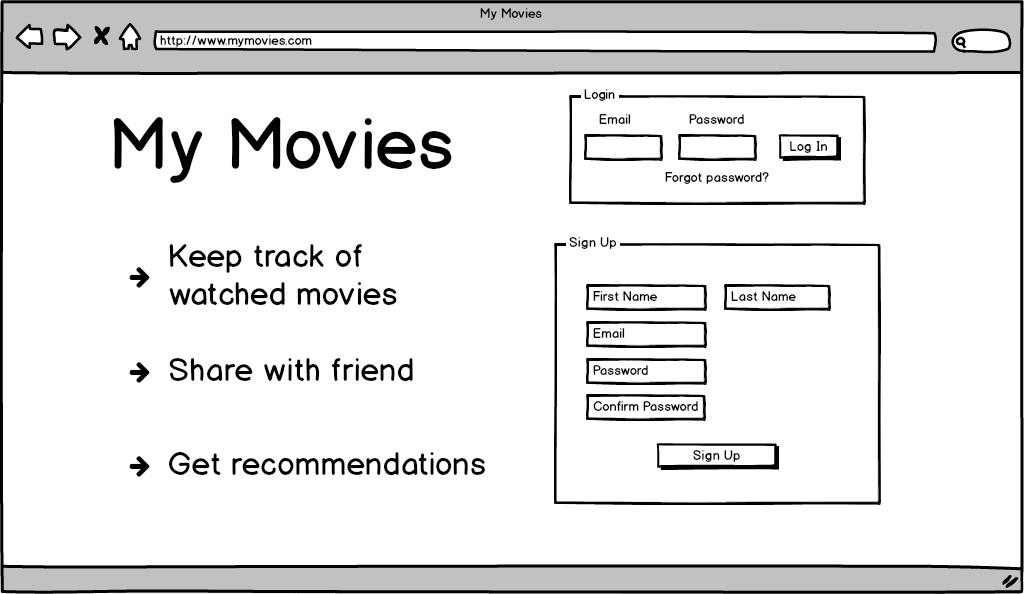
\includegraphics[width=0.8\textwidth]{fig/01-login.png}
\caption{\label{fig:login}Sign up / Login page.}
\end{figure}

After the login, the user is redirected to the timeline (Figure
\ref{fig:timeline}). On this screen there's a search field for finding movies
as well as friend. There's also a search field for marking movies as "watching
now". This is field is intended to be easily accessible. Three columns are
shown in this screen. The left column shows a few users statistics. The middle
column shows the timeline itself, featuring the recent friends' activity. The
right column presents a few movie tittles based on the system statistics as
well as movie premiere dates. This screen is highly inspired on
Facebook\cite{facebook} and Goodreads\cite{goodreads}.

\begin{figure}[!htb]
\centering
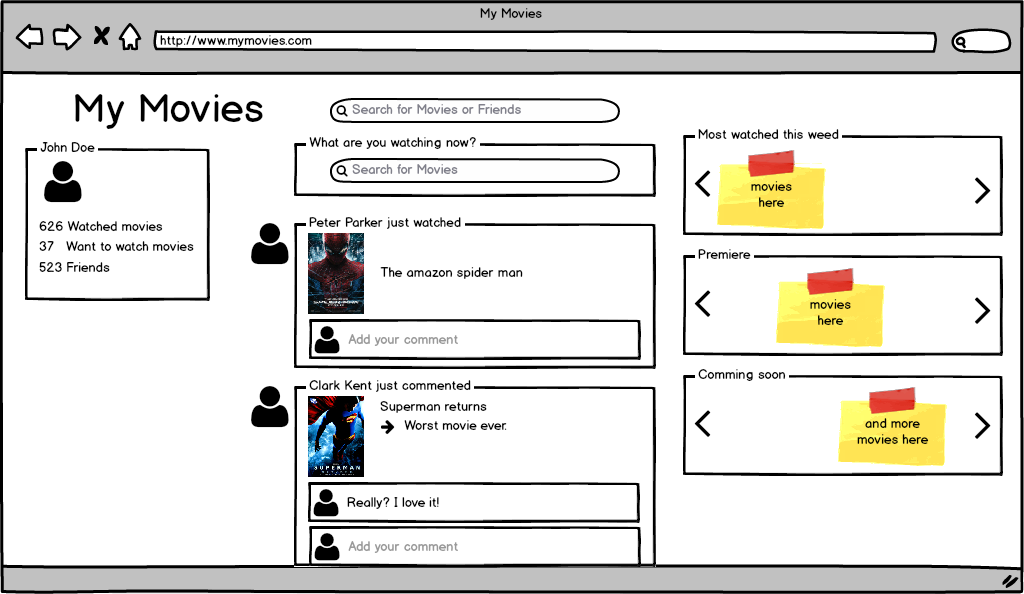
\includegraphics[width=0.8\textwidth]{fig/02-timeline.png}
\caption{\label{fig:timeline}Timeline.}
\end{figure}

Upon clicking a movie title (from the timeline of from the search field), the
user is redirected to the movie details page (Figure \ref{fig:movie}). This
screen shows some basic information from imdb, such as year, rating and
description, and also lists friends who watched it as well as comments from
friend. On this page the user can mark a movie as watched or "want to see".

\begin{figure}[!htb]
\centering
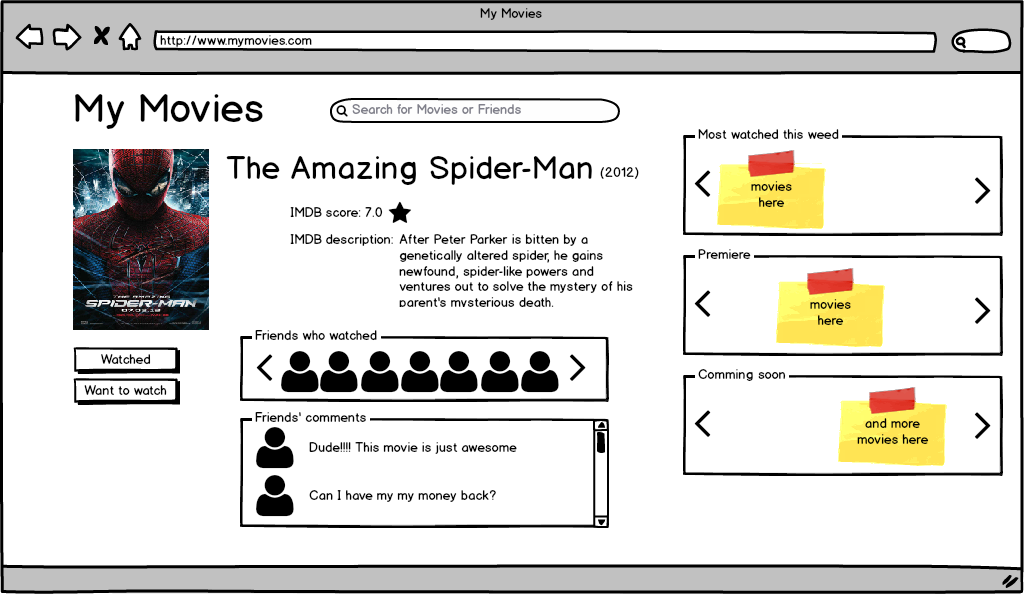
\includegraphics[width=0.8\textwidth]{fig/03-movie.png}
\caption{\label{fig:movie}Movie details page.}
\end{figure}

Upon clicking an user photo or name, the user is redirect to the user details
page (Figure \ref{fig:user}). This screen shows some user statistics on the
left side and lists their activity on the middle column. This page allows the
user to request friendship or start following someone.

\begin{figure}[!htb]
\centering
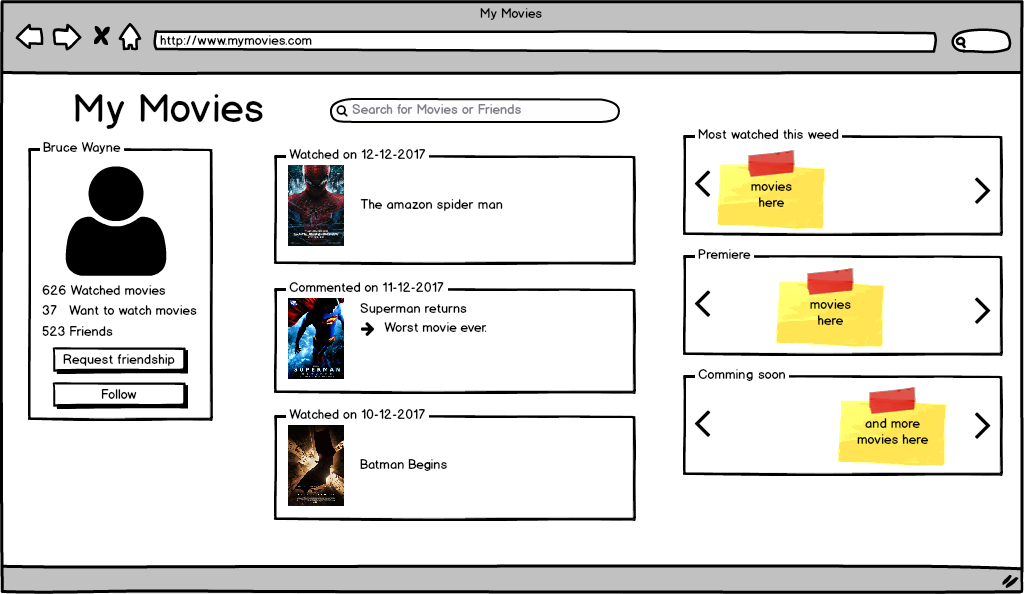
\includegraphics[width=0.8\textwidth]{fig/04-user.png}
\caption{\label{fig:user}User details page.}
\end{figure}

\bibliographystyle{plain}
\bibliography{bib}

%\label{sec:examples}
%
%\todo{Here's a comment in the margin!}
%\todo[inline, color=green!40]{This is an inline comment.}
%
%\begin{figure}
%\centering
%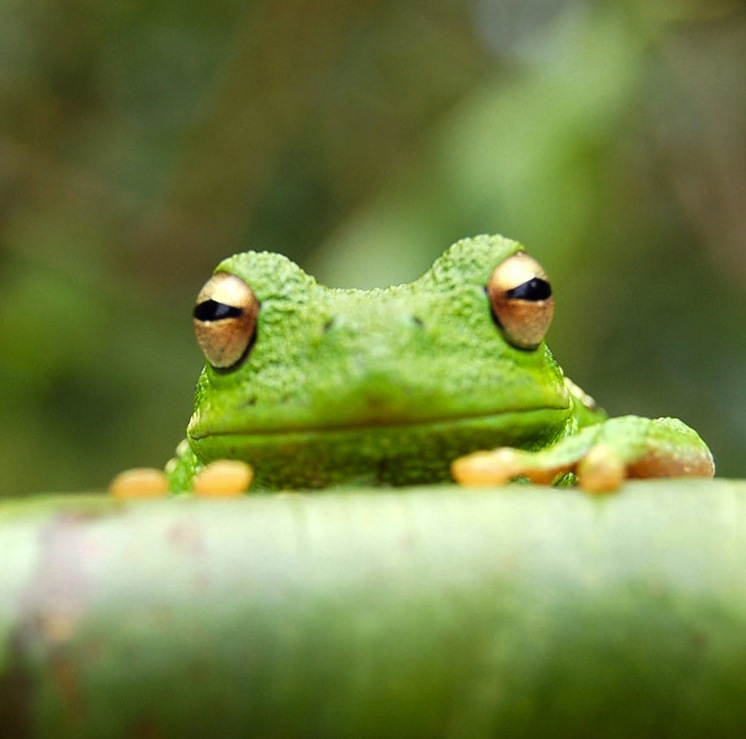
\includegraphics[width=0.5\textwidth]{frog.jpg}
%\caption{\label{fig:frog}This is a figure caption.}
%\end{figure}
%
%\begin{table}
%\centering
%\begin{tabular}{l|r}
%Item & Quantity \\\hline
%Widgets & 42 \\
%Gadgets & 13
%\end{tabular}
%\caption{\label{tab:widgets}An example table.}
%\end{table}
%
%\dots
%
%\begin{enumerate}
%\item Like this,
%\item and like this.
%\end{enumerate}
%\dots or bullet points \dots
%\begin{itemize}
%\item Like this,
%\item and like this.
%\end{itemize}

\end{document}
